

Pierwsze tomografy komputerowe przeżyły swój rozkwit w latach siedemdziesiątych ubiegłego wieku.
Spowodowało to, że obrazu medyczne nie były bezpośrednim wynikiem badania, a jedynie wynikiem obróbki danych pomiarowych przez komputer.
Dodatkowo obrazy przedstawiały przekroje, co sprawiły wiele trudności w ich interpretacji personelowi medycznemu.
Zwyczajne pliki graficzne (jak np. jpg, png, gif), nie nadawały się do zapisu takich obrazów, ponieważ zapisywały obraz w spektrum światła widzialnego, a konkretniej w postaci pozwalającej na odtworzenie światła widzialnego.
Natomiast obrazy medyczne sa zapisywanie w spektrum rentgenowskim.
Nie ułatwiał fakt, że każdy producent stosował inne metryki oraz inne oznaczenia swojego sprzętu.

\subsection{Standard DICOM v3.0}

Standard DICOM wersji trzeciej to standard definiujący ujednolicony sposób zapisu i przekazywania danych medycznych reprezentujących lub związanych z obrazami diagnostycznymi w medycynie.
Standard został wydany w 1993 przez dwie agencje ACR (American College of Radiology) i NEMA (National Electrical Manufactures Association).
Wcześniejsze wersje nazywały się ACR/NEMA v1.0, wydana w 1983 roku i ACR/NEMA v2.0, wydana w 1990 roku, stąd wersja trzecia.
Od wydania wersji trzeciej w 1993, standard jest wciąż rozwijany i uzupełniany o nowe elementy.
W obecnej chwili standard DICOM definiuje 81 różnych typów badań.

UWAGA: Za każdym razem kiedy jest odniesienie do obecnego standardu DICOM, w domyśle jest to odsłona 2019a.

\subsection{Sposób zapisu danych w pliku DICOM}

Plik w formacie DICOM przypomina bazę danych z rekordami.
Baza danych nazywa się \keyword{Data Set} i składa się z rekordów, które nazywają się \keyword{Data Element}.

\begin{figure}[!htbp]
    \caption{Wizualizacja ułożenia \keyword{Data Element}(wraz z budową) w \keyword{Data Set}}
    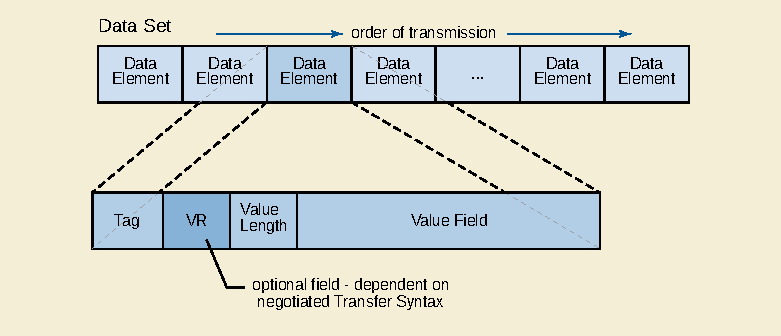
\includegraphics[]{img/dicom-dataelement001.pdf}
    \centering
    \label{fig:dicom-dataelement}
\end{figure}

\subsubsection{Data Element}

\keyword{Data Element} jest rekordem, który przechowuje jakaś jedną informacje o czymś.
Składa się z czterem elementów:

\begin{itemize}

    \item \keyword{Tag} - to unikalny identyfikator, złożony z dwóch liczb: grupy(uint16) i elementu(uint16) grupy.
    Informuje o tym co dany rekord w sobie zawiera.
    W jednym \keyword{Data Set} nie mogą się pojawić dwa \keyword{Data Element} posiadających ten sam \keyword{Tag}
    
    Obiekt reprezentujący \gdcmclass{Tag}.

    Na przykład: jeżeli liczby \keyword{Tag} przyjmą wartości odpowiednio wartość $0010_{16}$ i $0010_{16}$ to oznacza, że jest to tag \dicomtag{PatientName}{0010}{0010}, czyli zwiera w sobie parametr zawierają nazwę pacjenta.

    Dokładne omówienie \keyword{Tag}-ów znajduje się w sekcji \ref{sec:dicom-tag}.

    \item \keyword{Value Representation}, w skrócie \keyword{VR} – to dwa bajty w postaci tekstu, informujący o formacie w jaki parametr został zapisany.
    
    Dokładne omówienie \keyword{VR}-ów znajduje się w sekcji \ref{sec:dicom-vr}.

    \item \keyword{Value Length}, w skrócie \keyword{VL} - 32-bitowa lub 16-bitowa liczba nieoznaczona, która informuj o długości pola danych(\keyword{Value Field}).
    
    Wartość \keyword{VL} zwykle jest liczbą parzystą.
    Standard DICOM zakłada, że wszystkie dane powinny być dopełniane do parzystej ilości bajtów.
    
    \item \keyword{Value Field} (opcjonalne) - pole z parametrem o długości VL.
    
\end{itemize}

Wizualizacja budowy \keyword{Data Element} jest na rysunku \ref{fig:dicom-dataelement}.

\subsubsection{Tag}
\label{sec:dicom-tag}

Znacznik


\subsubsection{VR - Value Representation}
\label{sec:dicom-vr}

Reprezencaja wartości danej

Obiekt używany do przechowywania taga to \gdcmclass{VR}.
Na przykład: Decimal String, w skrócie DS, oznacza liczbę zapisaną za pomocą teksu.
Czasami to pole może być puste, wtedy należy się odnieść do VR przypisanego do taga, który określa standard.

\subsection{DICOMDIR}

coś o dicomdir